\documentclass{article}

% Use the geometry package to adjust margins
\usepackage[margin=1in]{geometry}
\usepackage{multicol} % For two-column layout
\usepackage{circuitikz}
\usepackage{enumitem}
\usepackage{caption}
\usepackage{float} % Add the float package
\usepackage{url}
\usepackage{mdframed}


% Remove section numbering and adjust formatting
\usepackage{titlesec}
\titleformat{\subsection}{\normalfont\large\bfseries}{}{0em}{}
\titleformat{\subsubsection}{\normalfont\normalsize\bfseries}{}{0em}{}

% Adjust the table of contents formatting
\usepackage{tocloft}
\renewcommand{\cftsecfont}{\normalfont}
\renewcommand{\cftsecpagefont}{\normalfont}
\renewcommand{\cftsecafterpnum}{\vspace{-0.5ex}}
\setlength{\cftbeforesecskip}{0.5ex}

\usepackage{lipsum} % For generating dummy text

\title{TESSA - Terrarium Environmental System with Smart Automation\\
	Documentation and Build Guide}
\author{Antonius Torode}
\date{\today}

\begin{document}
	
	\maketitle
	
	\tableofcontents
	
	%\listoffigures % If you have figures
	%\listoftables % If you have tables
	
	\begin{abstract}
		This project addresses the need for automated monitoring and periodic watering in a terrarium housing small geckos. The terrarium contains live plants and animals which will benefit from consistent monitoring of humidity and temperature. To ensure the geckos' well-being during extended absences, an automated system was developed to monitor and display environmental data. Additionally, the system includes a timer-based water dispensing mechanism for the plants and geckos. The project explores two implementations: one utilizing a Raspberry Pi and the other an Arduino Nano micro-controller. Both implementations involve the creation of a self-contained system adaptable to various scenarios, with a primary focus on automating environmental data display and periodic plant watering.
	\end{abstract}
	
		\hrule
		
		\section{Introduction}
		Recently, I acquired two small gecko's (I caught them roaming about my living room). I created a terrarium enclosure for them to live, where I have provided them with a few plants, live crickets for food, and a large hollowed rock which I keep full of water. Every now and then I spray down the plants (to give them water) as well as filling the water dish. Unfortunately with the approach of a long needed vacation, a need for automation arose. I cannot leave the water dish for the length of my trip without it evaporating and them running out of water. Therefore, I decided to create an automated system for keeping their water full and plants watered. This opportunity serves as the perfect one for re-learning some circuitry skills as well as developing them further.
		
		At the time of inception for this project, I had a few things laying around (including a Raspberry Pi). Therefore, a Raspberry Pi implementation was developed. With the desire to simplify the cost of the project as well as create a standalone system that doesn't rely on an OS, I explored using an Arduino Nano, and created an implementation using that as well. The primary goal of this project was both to automate and care for my gecko's enclosure while also furthering my skills and knowledge. It was decided (as I had never done it before) to create a complete integrated circuit (from a bare board and some pre-made components) for this project.
		
		\section{Project Overview}
		This is a simple project that utilizes an Arduino Nano (or a separate Raspberry Pi implementation) to setup an automated temperature/humidity monitoring for a terrarium as well as automating watering for filling a water dish and/or watering plants. The project involves created a self contained system. This system is highly versatile and the principals and components contained can be modified to fit a variety of situations and needs.

		For more project details, files, and a complete set of supplemental material - see the git repository here:
		\begin{mdframed}[backgroundcolor=gray!08, linewidth=1pt]
			https://github.com/torodean/Antonius-Personal/tree/master/TESSA
		\end{mdframed}
	
	\hrule

	\begin{multicols}{2} % Start two-column layout
		
		\section{Components and Materials}
		
		At the heart of this project, some sort of micro-controller will be needed (i.e. Arduino Nano). This will store the basic timing and control components for the various components. These components include a temperature and humidity sensor (DHT11), a submersible low voltage water pump, and a display for output (OLED). the setup for this type of system is highly configurable and therefore the components can also vary widely. Basic circuit components will also be needed.
		
		For testing the system, jumper cables and a breadboard are recommended. A complete components list is available for two various/possible setups.
		
		\subsubsection{Arduino Setup Components List}
		\begin{itemize}[itemsep=1pt, parsep=1pt]
			\item 1 Arduino Nano
			\item 1 DHT11 Sensor
			\item 1 SSD1306 OLED Display
			\item 1 micro 5V submersible pump
			\item 1 10k$\Omega$ resistor
			\item 1 diode (1N4001-1N4007)
			\item 1 2N 2222A Transistor (or similar NPN transistor)
			\item 1 10$\times$24 PCB
			\item Wires (varying sizes)
			\item Soldering kit (Solder Iron, Solder, Flux, etc)
		\end{itemize}
		
		\subsubsection{Raspberry Pi Setup Components List}
		\begin{itemize}[itemsep=1pt, parsep=1pt]
			\item 1 Raspberry Pi
			\item 1 DHT11 Sensor
			\item 1 SSD1306 OLED Display (optional)
			\item 1 micro 5V submersible pump
			\item 1 10k$\Omega$ resistor
			\item Wires (varying sizes)
			\item Jumper cables
		\end{itemize}
		
		
		\subsection{Component Descriptions}
		
		This project can be accomplished using many different components. Below is a list and description of some of the components used for this specific implementation. Some components have subtleties in how they should be implemented. It is recommended to read documentation on the components before using them.
		
		\subsubsection{DHT11}
		
		The DHT11 sensor is a low-cost and easy to use sensor for measuring temperature and humidity levels. The sensor provides digital output, making it easy to interface with micro-controllers like Arduino or Raspberry Pi. It uses a single wire to transmit two environmental data points in a single package. The DHT11 has the following features:			
		\begin{itemize}[itemsep=1pt, parsep=1pt]
			\item 3 to 5V power and I/O
			\item 2.5mA max current use during conversion (while requesting data)
			\item Good for 20-80\% humidity readings with 5\% accuracy
			\item Good for 0-50$^\circ$C temperature readings $\pm$2$^\circ$C accuracy
			\item No more than 1 Hz sampling rate (once every second)
			\item Body size 15.5mm $\times$ 12mm $\times$ 5.5mm
			\item 4 pins with 0.1" spacing
		\end{itemize}			
		
		\begin{minipage}{0.85\columnwidth} % Create a minipage that spans a single column
			\begin{figure}[H] 
				\centering % Center the figure horizontally
				\begin{circuitikz}
					% Draw the rectangle for DHT11
					\draw (0,0) rectangle (2,2) node[midway] {DHT11};
					
					% Draw pins on the right side
					\draw (2,1.7) -- ++(1,0) -- ++(0,1) node[draw, circle, minimum size=0.5cm, anchor=south] {5V}; % VCC
					\draw (2,1) -- ++(4,0) node[draw, circle, minimum size=0.5cm, anchor=west] {S}; % Data		
					\draw (5,1) -- (5,1.7) to [R, l=$10 \, \mathrm{k}\Omega$] (3,1.7);
					\draw (2,0.3) -- ++(1,0) node[ground] {}; % GND
				\end{circuitikz}
				\caption{\footnotesize The DHT11 circuit setup. The GND pin needs connected to ground. The 5V pin needs connected to a constant 5V DC source. The data pin needs connected to the proper data channel to read from. A $10\mathrm{k}\Omega$ resistor is connected between the data pin and voltage pin that serves as a `pull-up' for the data.}
				\label{fig:DHT11}
			\end{figure}
		\end{minipage}
		
		\subsubsection{Mini Submersible Water Pump}
		
		The pump I found for this project was a micro submersible mini water pump. It has the following features:			
		\begin{itemize}[itemsep=1pt, parsep=1pt]
			\item Rated voltage: 3.3V or 5V DC
			\item No load of water discharge capacity: 100L / H
			\item Load rated current: 150-250mA, Use: diving type
		\end{itemize}
		
		\begin{minipage}{0.85\columnwidth} % Create a minipage that spans a single column
			\begin{figure}[H] 
				\centering % Center the figure horizontally
				\begin{circuitikz}
					% Draw the rectangle for DHT11
					\draw (0,0) rectangle (2,1) node[midway] {Pump};
					
					% Draw pins on the right side
					\draw (2,0.7) -- ++(1.5,0) node[draw, circle, minimum size=0.5cm, anchor=west] {5V}; % VCC
					\draw (2,0.3) -- ++(1,0) node[ground] {}; % GND
				\end{circuitikz}
				\caption{\footnotesize The water pump only has two connectors, one for voltage, and the other for ground.}
				\label{fig:pump}
			\end{figure}
		\end{minipage}
		
		\subsubsection{SSD1306 I$^2$C OLED Display}
		
		The display I used for this project is a SSD1306 0.96 inch I$^2$C organic light-emitting diode (OLED) display. The OLED display doesn’t require a back light and the pixels only consume energy when on. The model I am using has 4 pins ($V_{in}$, GND, SCL, SDA). Some features of the display are as follows:
		\begin{itemize}[itemsep=1pt, parsep=1pt]
			\item Resolution: 128 x 64 dot matrix panel
			\item Support voltage: 3.3V-5V DC
			\item Wide range of operating temperature: -40$^\circ$C to 85$^\circ$C
			\item Embedded Driver IC: SSD1306. Communication: I2C/IIC Interface, only need two I / O ports
		\end{itemize}
		
		The I$^2$C driver means the bus consists of two signals: SDA and SCL. SDA (Serial Data) is the data signal and SCL (Serial Clock) is the clock signal.
		
		\begin{minipage}{0.85\columnwidth} % Create a minipage that spans a single column
			\begin{figure}[H] 
				\centering % Center the figure horizontally
				\begin{circuitikz}
					% Draw the rectangle for DHT11
					\draw (0,0) rectangle (2,2) node[midway] {OLED};
					
					% Draw pins on the right side
					\draw (0.3, 2) -- ++(0,0.5) -- ++(-0.5, 0) node[draw, circle, minimum size=0.5cm, anchor=east] {5V}; % VCC
					\draw (0.7, 2) -- ++(0,1) node[ground, rotate=180] {}; % GND
					\draw (1.3, 2) -- ++(0,1) -- ++(0.5,0) node[draw, circle, minimum size=0.5cm, anchor=west] {SCL};
					\draw (1.7, 2) -- ++(0,0.25) -- ++(1,0) node[draw, circle, minimum size=0.5cm, anchor=west] {SDA};
				\end{circuitikz}
				\caption{\footnotesize The OLED display has 4 inputs. The VCC is the power input, GND is ground, SDA is the serial data connector and SCL is the serial clock.}
				\label{fig:OLED}
			\end{figure}
		\end{minipage}
		
		\subsubsection{2N 2222A NPN Transistor}
		
		A transistor can be used as a switch by controlling the flow of current between its collector and emitter terminals. When a small current flows into the transistor's base terminal, it allows a larger current to pass from the collector to the emitter, effectively acting as an electronic switch that can be turned on and off based on the base current.
		
		\begin{minipage}{0.85\columnwidth} % Create a minipage that spans a single column
			\begin{figure}[H] 
				\centering % Center the figure horizontally
				\begin{circuitikz}
					% Transistor
					\draw (0,0) node[npn, anchor=E] (npn) {}; % Anchor at the emitter (E)
					
					\draw (npn.C) node[left] {C};
					\draw (npn.E) node[left] {E};
					\draw (npn.B) node[above] {B};
					
					\draw (npn.C) -- ++(0,1) node[draw, circle, minimum size=0.5cm, anchor=south] {5V}; 
					\draw (npn.E) -- ++(0,-1) node[draw, circle, minimum size=0.5cm, anchor=north] {OUT};
					\draw (npn.B) -- ++(-1,0) node[draw, circle, minimum size=0.5cm, anchor=east] {IN}; 
				\end{circuitikz}
				\caption{\footnotesize The 2N 2222A NPN Transistor. The IN is the triggering 3.3V input signal. The OUT is connected to the device being powered and is activated when the IN voltage is powered on. A common ground should be used among the connected components.}
				\label{fig:Transistor}
			\end{figure}
		\end{minipage}
		
		
		\subsubsection{Arduino Nano}
		
		The Arduino Nano is a compact and versatile micro-controller board designed for embedded electronics projects and prototyping. The Nano is known for its small physical size, making it suitable for applications with limited space or when a compact design is essential. The Nano includes a set of digital and analog pins, allowing you to interface with sensors, actuators, and other electronic components. These pins can be programmed for input or output. It features a USB connector for easy programming and communication with a computer. This makes it convenient for uploading code and debugging. It is programmed using the Arduino IDE, which provides a user-friendly interface for writing, uploading, and debugging code. A large community and extensive libraries are available to simplify development. Like other Arduino boards, the Nano is open-source hardware and software. This means that the design files, schematics, and software are freely available for modification and customization.
		
		Some features of the arduino nano that are important for this project are as follows:
		\begin{itemize}[itemsep=1pt, parsep=1pt]
			\item High-performance low-power 8-bit processor
			\item Has a 5V DC output pin.
			\item Has multiple programmable I/O pins.
			\item Has SDA and SCL connections for I$^2$C communication.
		\end{itemize}
		
		\subsubsection{Raspberry Pi}
		
		The Raspberry Pi is a versatile and powerful single-board computer designed for various computing and electronics projects. The Raspberry Pi is equipped with a high-performance ARM-based\footnote{This is important because the newer versions of the Arduino IDE are not pre-built for the ARM architecture.} processor (varies by model) that provides the processing power needed for a wide range of applications. It features a set of General-Purpose Input/Output (GPIO) pins, which can be programmed for digital input and output as well as hardware interfacing. These pins are crucial for connecting sensors, actuators, and other components. The Raspberry Pi supports communication protocols like I$^2$C and SPI, allowing you to connect and communicate with a variety of sensors and devices easily. Like Arduino, the Raspberry Pi is open-source hardware and software. It has a large and active community that offers support, tutorials, and a wide range of software packages.
		
		Some Raspberry Pi models include built-in Wi-Fi and Bluetooth capabilities, making wireless communication and IoT projects convenient. The Raspberry Pi has an HDMI output for connecting to displays, making it suitable for applications that require visual feedback. Between these two features, a lot of possibilities open up with allowing the DHT11 sensor to be displayed on Pi screen rather than an OLED as well as potentially being able to monitor it remotely.
		
		Some features of the Raspberry Pi has that are important for this project are as follows:
		\begin{itemize}[itemsep=1pt, parsep=1pt]
			\item Has a 5V DC output pin.
			\item Has multiple programmable GPIO pins.
			\item Has SDA and SCL connections for I$^2$C communication.
		\end{itemize}
		
		\section{System Architecture}
		Given the two approaches outlined below for this project, there are a few things of importance to note when setting up and working with the various components. For the Raspberry Pi implementation, I used an Ubuntu 22.04.2 LTS install. Using the Raspian OS, things may vary slightly but shouldn't differ much.
		
		When working with and programming the Arduino Nano, I used the Raspberry Pi system as my working/development machine. As an afterthought, this is not recommended. The Raspberry Pi uses an ARM processor architecture which requires a few extra steps for setting up the Arduino IDE. After setting this up on a separate laptop, it was much easier to get things going (as well as things working a lot faster on a faster machine) as far as setup and development.
		
		\section{Raspberry Pi Implementation}
		
		\subsection{Circuit Diagram and Wiring}
		See figure \ref{fig:Raspberry Pi Setup} in section \ref{appendix:schematics}.
		
		\subsection{Software Setup}
		
		\begin{enumerate}
			\item Setup and Install Python3 for development
			\begin{itemize}
				\item sudo apt-get install python3
				\item sudo apt-get install python3-pip
				\item sudo apt-get install build-essential python3-dev
			\end{itemize}
			\item Setup and Install git
			\begin{itemize}
				\item sudo apt-get install git-core
			\end{itemize}
			\item Install DHT11 Drivers
			\begin{itemize}
				\item git clone https://github.com/adafruit/ Adafruit\_Python\_DHT.git
				\item cd Adafruit\_Python\_DHT
				\item sudo python3 setup.py install
			\end{itemize}
			\item Install OLED Drivers
			\begin{itemize}
				\item \textbf{THIS SECTION IN PROGRESS.}
				\item sudo python3 setup.py install
			\end{itemize}
		\end{enumerate}
		
		\subsection{Python Code}
		For testing, two separate programs were created. One which tests the DHT11 sensor and displays the output to the OLED and one which tests the pump timing. After these were working, another python script was made which combines these functions into one script. These can all be seen in section \ref{appendix:code}.
		
		\subsection{Testing and Troubleshooting}
		I did not really experience any issues with this setup, so I have no troubleshooting advice to give here.
		
		\section{Arduino Nano Implementation}
		This is the implementation using the Arduino Nano as the micro-controller. This setup is completely standalone and does not require a desktop monitor hookup once finished. Rather, it displays all the information on the OLED display and runs the pump based on a pre-programmed timer. A separate machine will be required to program the Arduino Nano. I recommend using a laptop or desktop running Linux (I have not tried this on a windows machine). If a Raspberry Pi is used as the development machine (this is what I used), a few extra steps will be needed to get the Arduino IDE software functioning. 
		
		\subsection{Circuit Diagram and Wiring}
		See figure \ref{fig:Arduino Nano Setup} in section \ref{appendix:schematics}.
		
		\subsection{Software Setup}
		\begin{enumerate}
			\item Install Arduino IDE
			\begin{itemize}
				\item The steps for this will vary depending on the development machine.
			\end{itemize}
			\item Install DHT11 Drivers
			\begin{itemize}
				\item This should show as ``" in the Arduino IDE Library Manager
			\end{itemize}
			\item Install SSD1306 Drivers
			\begin{itemize}
				\item This should show as ``Adafruit SSD1306" in the Arduino IDE Library Manager
			\end{itemize}
		\end{enumerate}
		
		\subsection{Arduino Code}
		For testing, three separate programs were created. One which tests the OLED display on it's own, one which tests the DHT11 sensor and displays the output to the OLED and one which tests the pump timing. After these were working, another script was made which combines these functions into one script. These can all be seen in section \ref{appendix:code}.
		
		\subsection{Testing and Troubleshooting}
		If you are testing the setup using a breadboard, I recommend making sure the Arduino Nano jumper pins (at least the ones being used) are soldered on. If they are not soldered on, some of the jumper pins may not have a good connection and things can work unexpectedly.
		
		\section{3D Printed Enclosure}
		At the time of creating this project, no 3D printed enclosure was designed. This is, however, a plan for the future to keep everything protected and enclosed.
		
		\section{Power Supply}
		For the Raspberry Pi implementation, all power comes from the Raspberry Pi itself, therefore no extra power sources are needed\footnote{If this project is adapted to use a more powerful pump, this will of course change.}. For the Arduino Nano implementation, the power comes from a dedicated USB powered cable. This can be accomplished in any of the usual ways that a USB device is charged (I would not recommend trying fast chargers as I have no tested with any of those).
		
		\section{Usage and Operation}
		\textbf{THIS SECTION IN PROGRESS.}
		
		\section{Maintenance and Troubleshooting}
		\textbf{THIS SECTION IN PROGRESS.}
		
		\section{Full Enclosure Setup}		
		The complete setup and implementation will vary for every setup. This is simply what I have used and designed for my specific setup and needs.
		
			\subsection{Equipment and Tools}
			\textbf{THIS SECTION IN PROGRESS.}
			
			\subsection{Setup and Implementation}
			\textbf{THIS SECTION IN PROGRESS.}
		
		\section{Future Enhancements}
		There are many additions or future enhancements that can be made to this system. These can include (but are not limited to) the following:
		\begin{itemize}
			\item Add in an override switch for activating the pump outside of the normal programmed timing for the Arduino Nano setup.
			\item External monitoring for the Arduino implementation would be nice. Perhaps some sort of wireless signal output that can be monitored to display status messaging.
		\end{itemize}
		
		\section{Author Contact Information}
		
		If you have any questions or comments about this project, you can find the authors contact information on his website at the following link:
		
		\begin{mdframed}[backgroundcolor=gray!08, linewidth=1pt]
			\url{https://torodean.github.io}
		\end{mdframed}
		
	\end{multicols} % End two-column layout	
	
	\begin{thebibliography}{X}
		\bibitem{DHT11} DHT11: https://www.adafruit.com/product/386
		\bibitem{SSD1306_datasheet} SSD1306 Datasheet: https://cdn-shop.adafruit.com/datasheets/SSD1306.pdf
		\bibitem{arduino nano} Arduino Nano: https://docs.arduino.cc/hardware/nano
	\end{thebibliography}	
	
	\section{Appendices}
	These Appendices include extra data and supplemental material for the sections above.
	
	\subsection{Appendix A: Bill of Materials}
	Most of the components for this project were purchased in kits of other components. Therefore, this is an approximate (overestimate in most cases) cost of components for items used in this project. 
	
	\begin{multicols}{2}
		\begin{itemize}
			\item Raspberry Pi Implementation
			\begin{itemize}
				\item Raspberry Pi 4: \$70
				\item Mini Water Pump: \$2
				\item DHT11 sensor: \$2
				\item (optional) OLED display: \$3
				\item Jumper Cables/wiring: \$2
				\item Resistor/Transistor/Diode: \$1
				\item Breadboard: \$3
				\item \textbf{Total: \$83}
			\end{itemize}
			
			\columnbreak
			
			\item Arduino Nano Implementation
			\begin{itemize}
				\item Arduino Nano V3.0: \$6
				\item Mini Water Pump: \$2
				\item DHT11 sensor: \$2
				\item OLED display: \$3
				\item 10$\times$24 blank PCB: \$1
				\item Jumper Cables/wiring: \$2
				\item Resistor/Transistor/Diode: \$1
				\item (optional for testing) Breadboard: \$3
				\item Soldering iron, wire cutters, solder, flux, etc: Variable
				\item \textbf{Total: \$20}
			\end{itemize}
		\end{itemize}
	\end{multicols}
	
	\subsection{Appendix B: Schematics and PCB Designs \label{appendix:schematics}}
	
	\subsubsection{Arduino Nano Circuit Design}
	\begin{figure}[H] 
		\centering % Center the figure horizontally
		\begin{circuitikz}
			% Draw the rectangle for DHT11
			\draw (0,0) rectangle (2,2) node[midway] {DHT11};
			
			\node[draw, circle, minimum size=0.5cm] (power) at (3,3) {5V};
			\node[draw, rectangle, minimum width=2cm, minimum height=1cm] (pump) at (12,2.8) {Pump};
			\node[draw, rectangle, minimum width=2cm, minimum height=2cm] (oled) at (8,-2) {OLED};
			
			% Power
			\draw (2,1.7) -- (3,1.7) -- (power.south); % VCC
			
			% DHT11
			\draw (2,1) -- ++(3.5,0) node[draw, circle, minimum size=0.5cm, anchor=west] {11}; % Data		
			\draw (5,1) -- (5,1.7) to [R, l=$10 \, \mathrm{k}\Omega$] (3,1.7);
			\draw (2,0.3) -- ++(1,0) node[ground] {}; % GND
			
			% Transistor
			\draw (10,3) node[npn, anchor=E, rotate=90] (npn) {}; % Anchor at the emitter (E)
			
			% Transistor Labels
			\draw (npn.C) node[above] {C};
			\draw (npn.E) node[above] {E};
			\draw (npn.B) node[left] {B};
			
			% Transistor Connectors
			\draw (npn.C) -- (power.east); % Collector to Vcc
			\draw (npn.E) -- (11,3);
			\draw (npn.B) -- ++(0,-0.8) node[draw, circle, minimum size=0.5cm, anchor=north] {12}; 
			
			% OLED connectors.		
			\draw (7.3,-1) -- (7.3,3); % GND
			\draw (7.8,-1) -- ++(0,1) node[ground, rotate=180] {}; % GND		
			\draw (8.3,-1) -- ++(0,1) -- ++(1.5,0) node[draw, circle, minimum size=0.5cm, anchor=west] {A5};
			\draw (8.7,-1) -- ++(0,0.25) -- ++(2,0) node[draw, circle, minimum size=0.5cm, anchor=west] {A4};
			
			\draw (11,2.6) -- ++(-0.3, 0) -- ++(0, -0.5) node[ground]{};
		\end{circuitikz}
		\caption{\footnotesize The Circuit diagram for the Arduino Nano setup. All grounds must be common. The A4 and A5 pins correspond to the Arduino Nano's SDA/SCL pins and should not be modified. The other circle connectors 11 and 12 correspond to the I/O pins on the Nano and can be changed to any of the other I/O pins if desired (the code and circuitry would need updated appropriately).}
		\label{fig:Arduino Nano Setup}
	\end{figure}

	\subsubsection{Arduino Nano Circuit Design With Extra Pump(s)}
	\begin{figure}[H] 
		\centering % Center the figure horizontally
		\begin{circuitikz}
			% Draw the rectangle for DHT11
			\draw (0,0) rectangle (2,2) node[midway] {DHT11};
			
			\node[draw, circle, minimum size=0.5cm] (power) at (3,3) {5V};
			\node[draw, rectangle, minimum width=2cm, minimum height=1cm] (pump) at (12,2.8) {Pump 1};			
			\node[draw, rectangle, minimum width=2cm, minimum height=1cm] (pump2) at (12,0.3) {Pump 2};
			\node[draw, rectangle, minimum width=2cm, minimum height=2cm] (oled) at (8,-4.5) {OLED};
			
			% Power
			\draw (2,1.7) -- (3,1.7) -- (power.south); % VCC
			
			% DHT11
			\draw (2,1) -- ++(3.5,0) node[draw, circle, minimum size=0.5cm, anchor=west] {11}; % Data		
			\draw (5,1) -- (5,1.7) to [R, l=$10 \, \mathrm{k}\Omega$] (3,1.7);
			\draw (2,0.3) -- ++(1,0) node[ground] {}; % GND
			
			% Transistors
			\draw (10,3) node[npn, anchor=E, rotate=90] (npn) {}; % Anchor at the emitter (E)
			\draw (10,0.5) node[npn, anchor=E, rotate=90] (npn2) {}; % Anchor at the emitter (E)
			
			% Transistor Labels
			\draw (npn.C) node[above] {C};
			\draw (npn.E) node[above] {E};
			\draw (npn.B) node[left] {B};
			
			% Transistor Labels
			\draw (npn2.C) node[above] {C};
			\draw (npn2.E) node[above] {E};
			\draw (npn2.B) node[left] {B};
			
			% Transistor Connectors
			\draw (npn.C) -- (power.east); % Collector to Vcc
			\draw (npn.E) -- (11,3);
			\draw (npn.B) -- ++(0,-0.5) node[draw, circle, minimum size=0.5cm, anchor=north] {12}; 
			
			% Transistor Connectors
			\draw (npn2.C) -- (7.3,0.5); % Collector to Vcc
			\draw (npn2.E) -- (11,0.5);
			\draw (npn2.B) -- ++(0,-0.5) node[draw, circle, minimum size=0.5cm, anchor=north] {10}; 
			
			% OLED connectors.		
			\draw (7.3,-3.5) -- (7.3,3); % GND
			\draw (7.8,-3.5) -- ++(0,1) node[ground, rotate=180] {}; % GND		
			\draw (8.3,-3.5) -- ++(0,1) -- ++(1.5,0) node[draw, circle, minimum size=0.5cm, anchor=west] {A5};
			\draw (8.7,-3.5) -- ++(0,0.25) -- ++(2,0) node[draw, circle, minimum size=0.5cm, anchor=west] {A4};
			
			\draw (11,2.6) -- ++(-0.3, 0) -- ++(0, -0.5) node[ground]{};
		\end{circuitikz}
		\caption{\footnotesize The Circuit diagram for the Arduino Nano setup. All grounds must be common. The A4 and A5 pins correspond to the Arduino Nano's SDA/SCL pins and should not be modified. The other circle connectors 10, 11 and 12 correspond to the I/O pins on the Nano and can be changed to any of the other I/O pins if desired (the code and circuitry would need updated appropriately).}
		\label{fig:Arduino Nano Setup}
	\end{figure}

	\subsubsection{Raspberry Pi Circuit Design}
	\begin{figure}[H] 
		\centering % Center the figure horizontally
		\begin{circuitikz}
			% Draw the rectangle for DHT11
			\draw (0,0) rectangle (2,2) node[midway] {DHT11};
			
			\node[draw, circle, minimum size=0.5cm] (power) at (3,3) {5V};
			\node[draw, rectangle, minimum width=2cm, minimum height=1cm] (pump) at (12,2.8) {Pump};
			\node[draw, rectangle, minimum width=2cm, minimum height=2cm] (oled) at (8,-3) {OLED};
			
			% Power
			\draw (2,1.7) -- (3,1.7) -- (power.south); % VCC
			
			% DHT11
			\draw (2,1) -- ++(3.5,0) node[draw, circle, minimum size=0.5cm, anchor=west] {17}; % Data		
			\draw (5,1) -- (5,1.7) to [R, l=$10 \, \mathrm{k}\Omega$] (3,1.7);
			\draw (2,0.3) -- ++(1,0) node[ground] {}; % GND
			
			% Transistor
			\draw (10,3) node[npn, anchor=E, rotate=90] (npn) {}; % Anchor at the emitter (E)
			
			% Transistor Labels
			\draw (npn.C) node[above] {C};
			\draw (npn.E) node[above] {E};
			\draw (npn.B) node[left] {B};
			
			% Transistor Connectors
			\draw (npn.C) -- (power.east); % Collector to Vcc
			\draw (npn.E) -- (11,3);
			\draw (npn.B) -- ++(0,-0.8) node[draw, circle, minimum size=0.5cm, anchor=north] {18}; 
			
						% OLED connectors.		
			\draw (7.3,-2) -- (7.3,3); % GND
			\draw (7.8,-2) -- ++(0,1) node[ground, rotate=180] {}; % GND		
			\draw (8.3,-2) -- ++(0,1) -- ++(1.5,0) node[draw, circle, minimum size=0.5cm, anchor=west] {2};
			\draw (8.7,-2) -- ++(0,0.25) -- ++(2,0) node[draw, circle, minimum size=0.5cm, anchor=west] {3};
			
			\draw (11,2.6) -- ++(-0.3, 0) -- ++(0, -0.5) node[ground]{};
			
			\draw[dotted] (6,0) -- (6,-4.3) -- (12,-4.3) -- (12,0) -- (6,0);
			
			\draw (10.5, -3) node[]{OPTIONAL};
			\draw (10.5, -3.5) node[]{OLED};
		\end{circuitikz}
		\caption{\footnotesize The Circuit diagram for the Raspberry Pi setup. All grounds must be common. The OLED section is optional and can be omitted if the user would rather monitor from the same display as the Raspberry Pi. the circles with numbers correspond to the GPIO pins on the Raspberry Pi. Pins 2 and 3 are the SDA/SCL pins respectively and should be kept as they are but the others can be used with other GPIO pins if desired (the code will need updated appropriately).}
		\label{fig:Raspberry Pi Setup}
	\end{figure}	
	
	\subsection{Appendix C: Code Samples \label{appendix:code}}
	
		\subsubsection{Raspberry Pi Python Code}
		\textbf{THIS SECTION IN PROGRESS.}
		
		\subsubsection{Arduino Nano Code}
		\textbf{THIS SECTION IN PROGRESS.}
	
	\subsection{Appendix D: 3D Printing Files}
	\textbf{THIS SECTION IN PROGRESS.}
	
	\subsection{Appendix E: Micro-Controller Pin Diagrams}
	
	\subsubsection{Arduino Nano Pinout}
	
	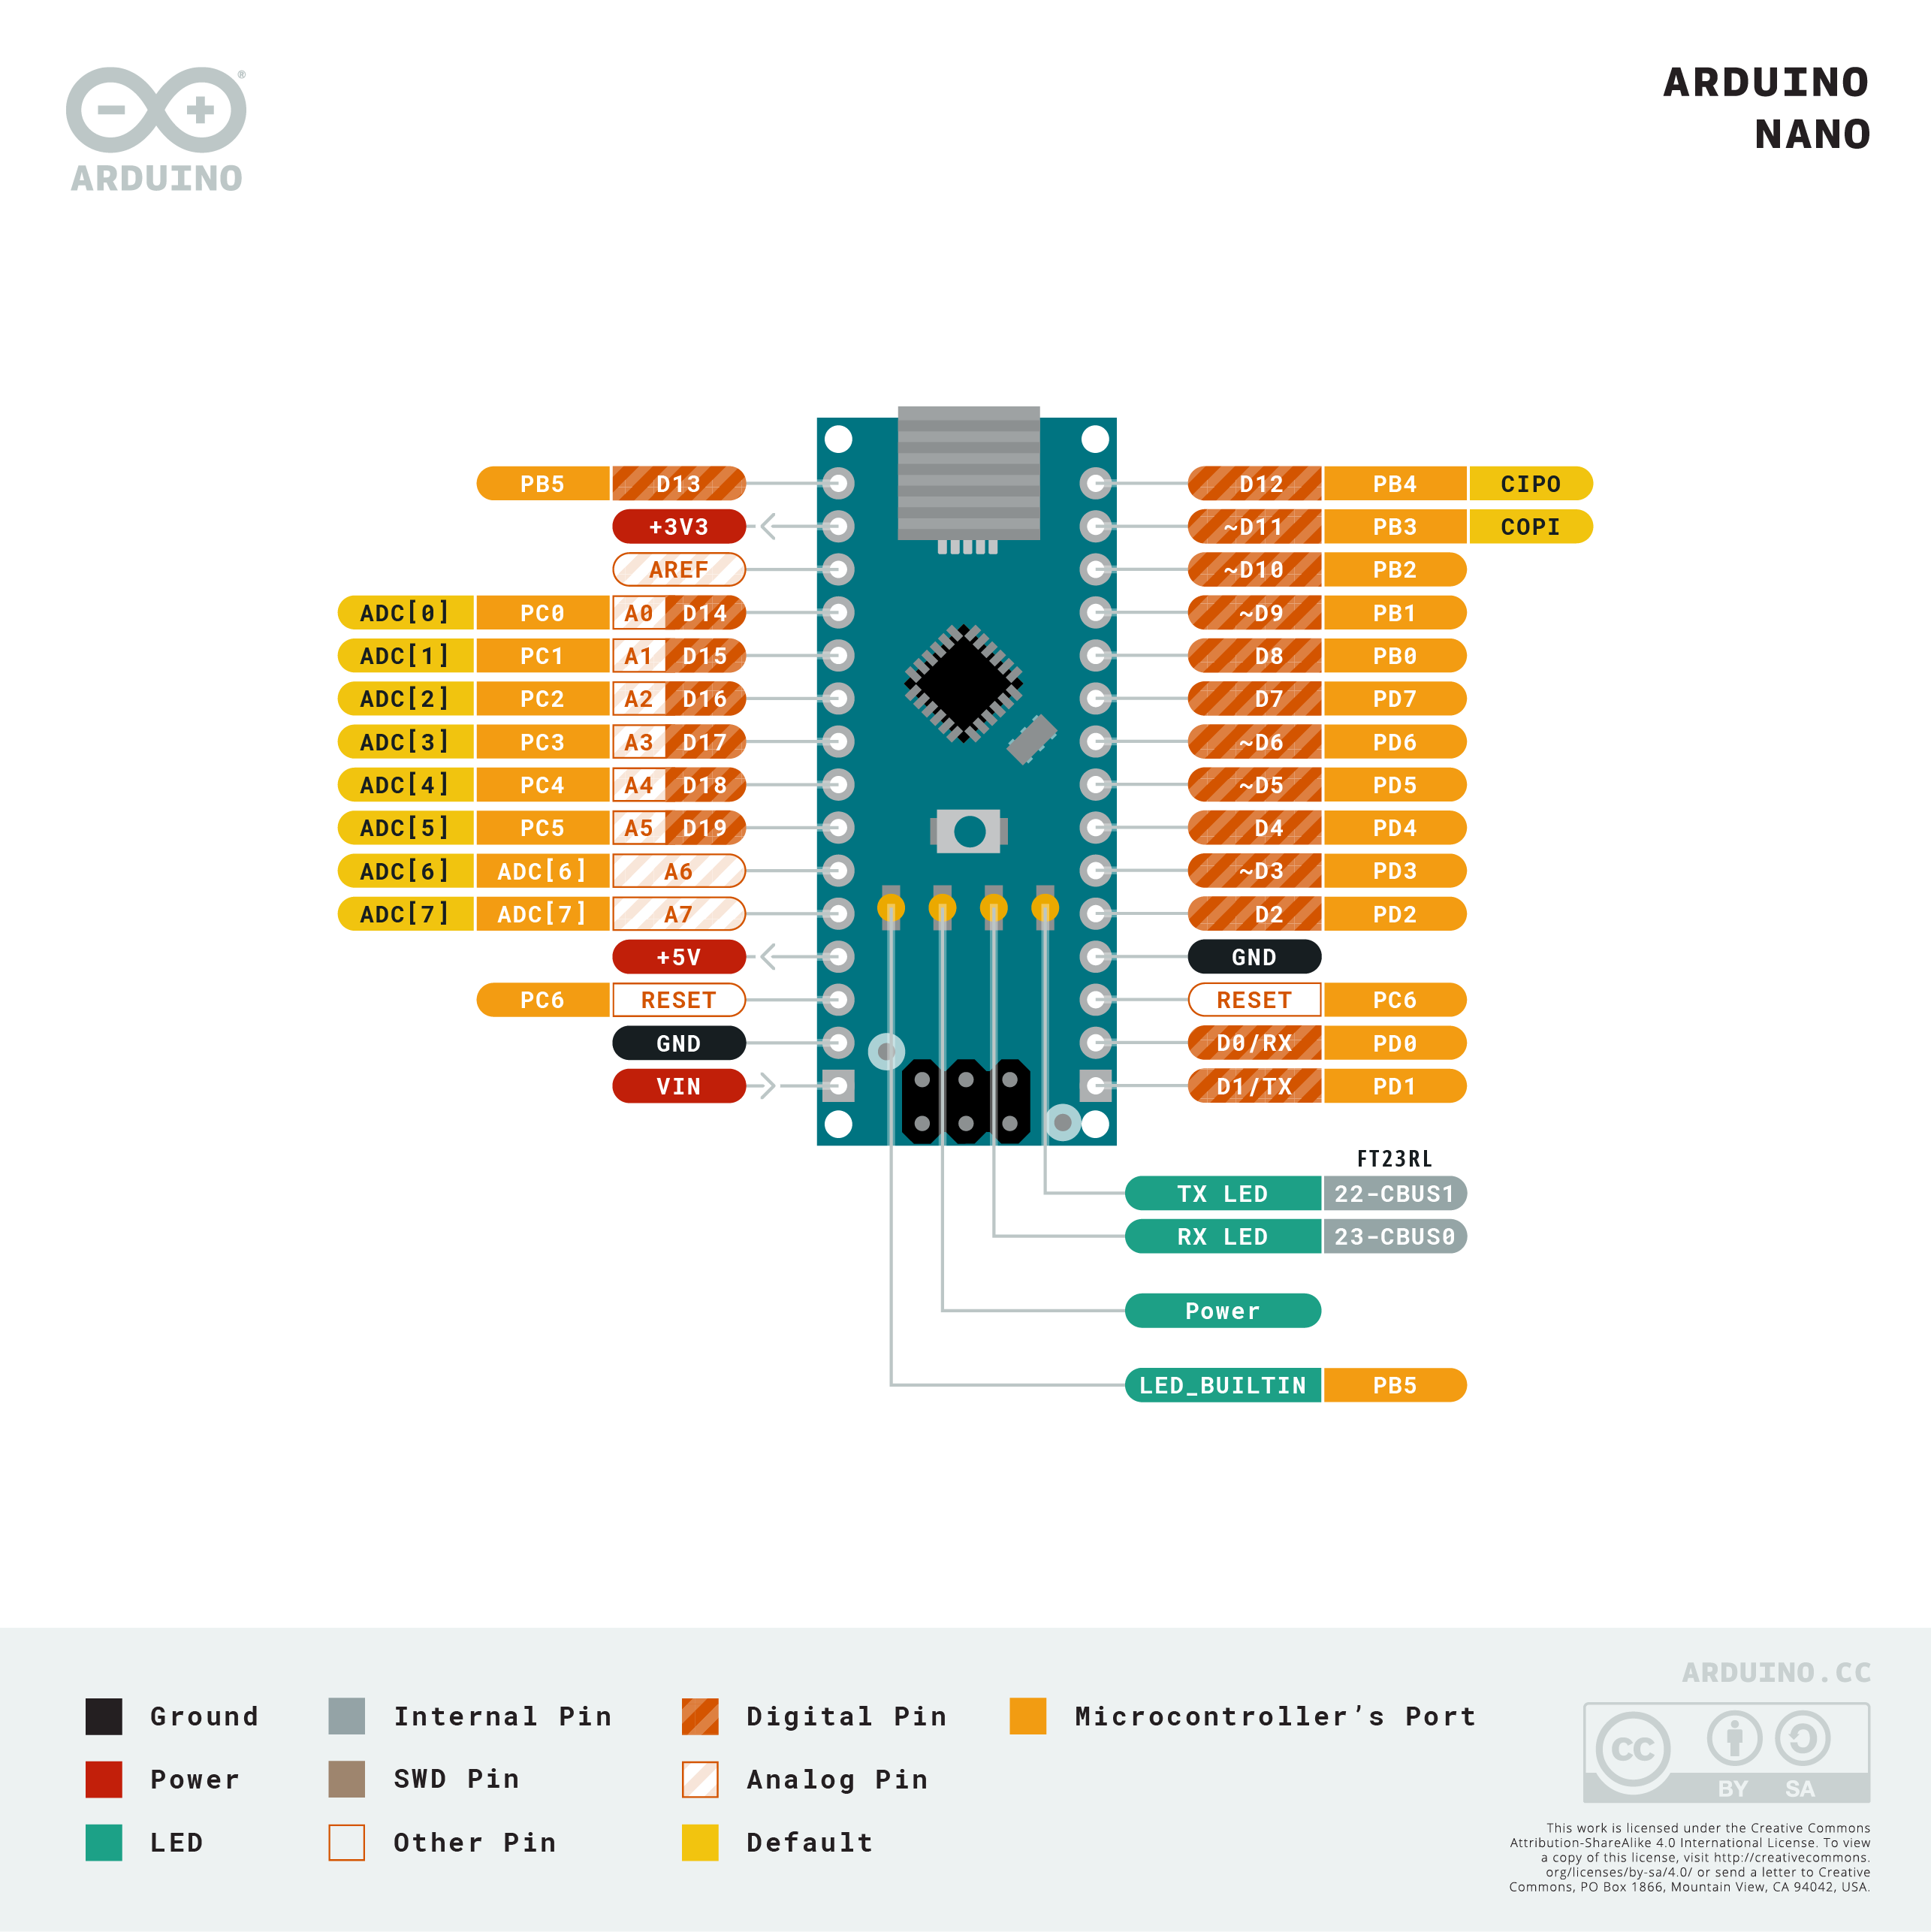
\includegraphics[width=\linewidth]{A000005-pinout}
		
		\subsubsection{Raspberry Pi Pinout}
	
	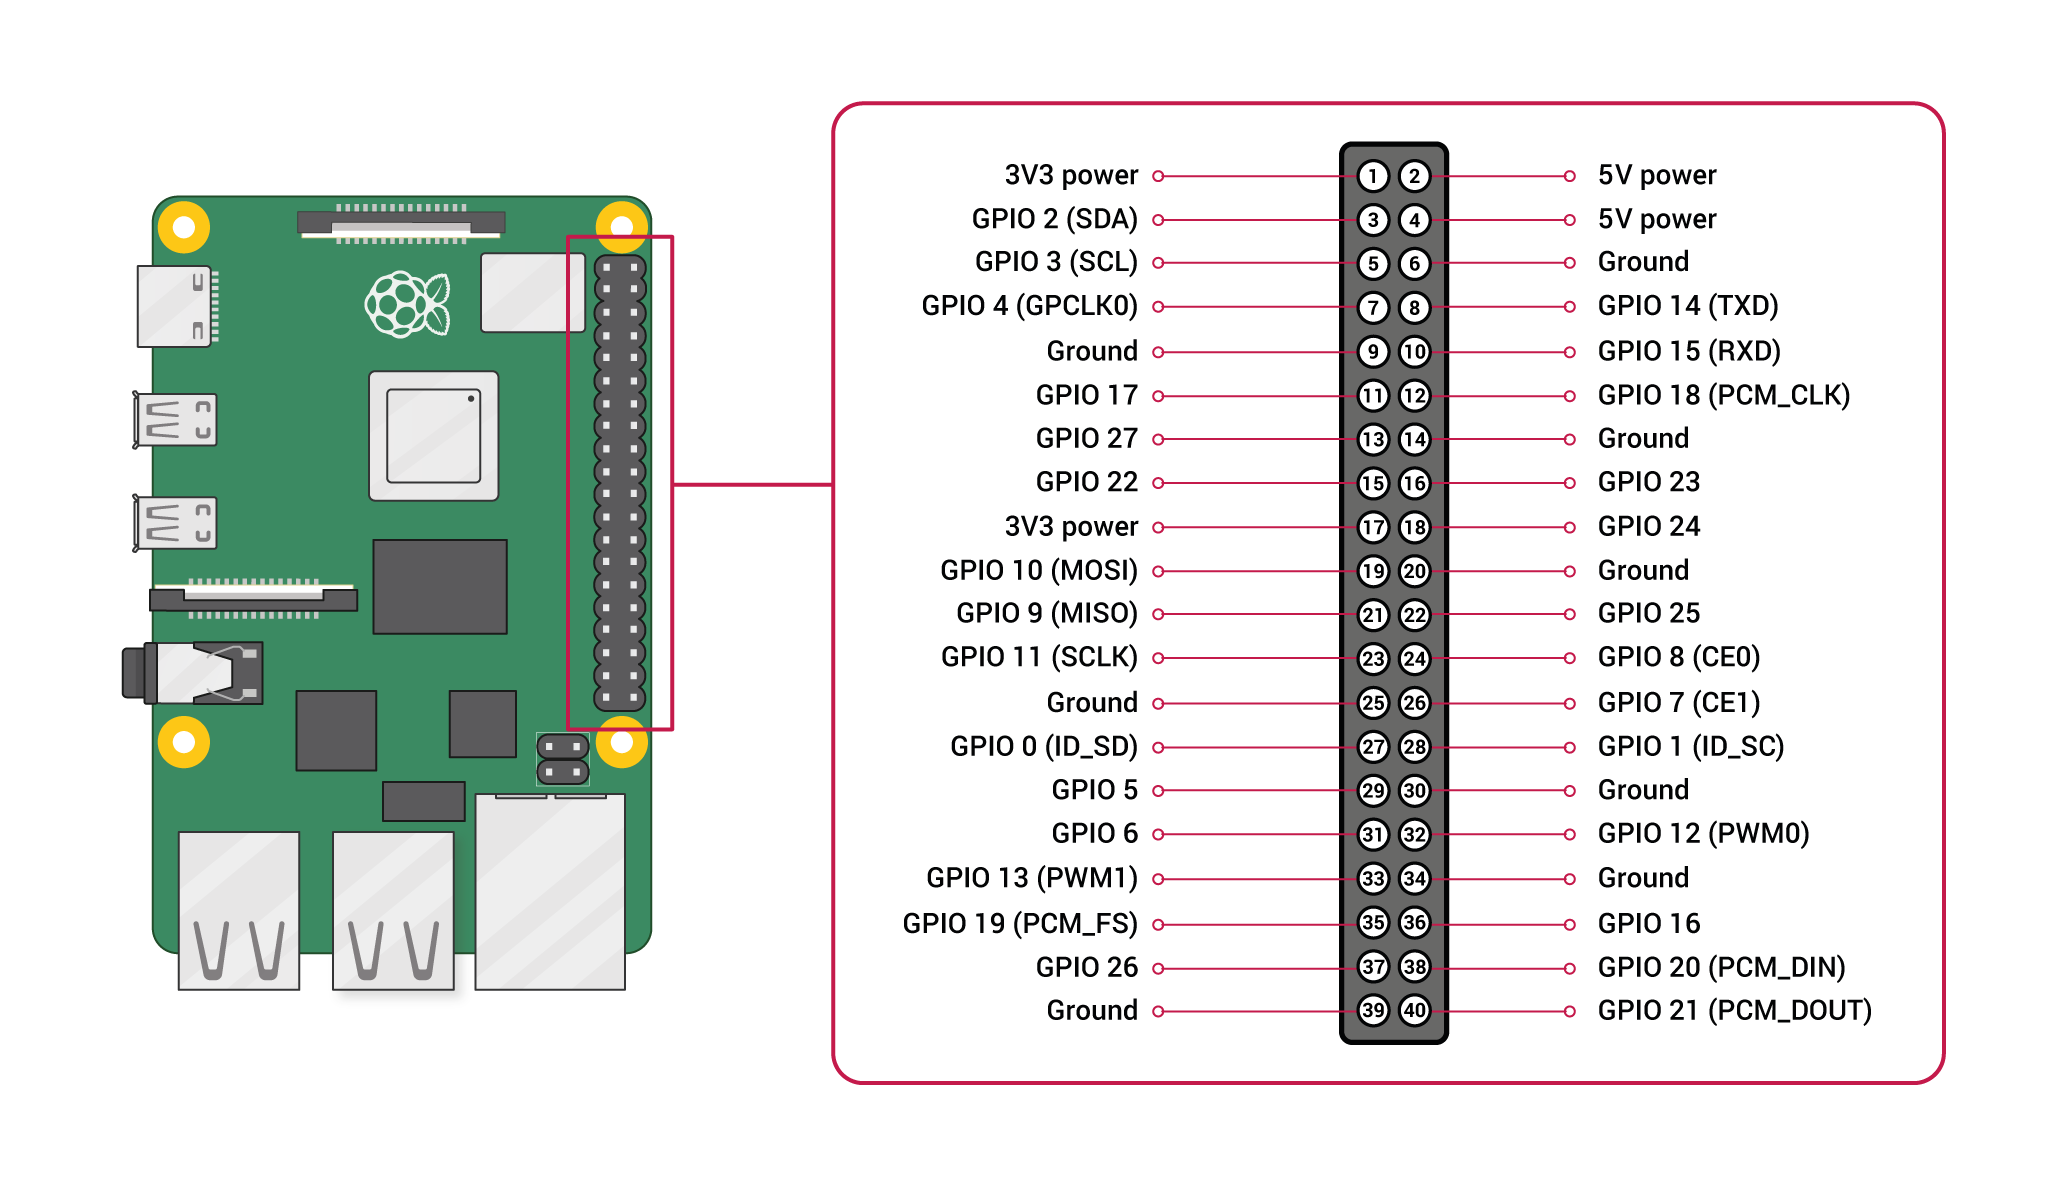
\includegraphics[width=\linewidth]{GPIO-Pinout-Diagram-2}
	
\end{document}
